\textbf{Decomposi\c c\~ao STL}
através da decomposição, é possível analisar se a série apresenta tendência, sazonalidade e resíduos. Ao observar a Figura \ref{fig:stl}, é evidente que os dados exibem ambos os padrões. Isso indica que a série é estacionária, como confirmado pelo seguinte teste ADF anterior.

%\begin{figure}[!htb]
%	\centering
%	\caption{Decomposição STL aditiva dos dados coletados}
%	\label{fig:stl-aditiva}
%	\includegraphics[width=1\linewidth]{"Resultados/Figuras/STL aditiva"}
%	
%	
%\end{figure}

\begin{figure}[!htb]
	\centering
	\caption{Decomposição STL aditiva dos dados coletados}
	\label{fig:stl}
	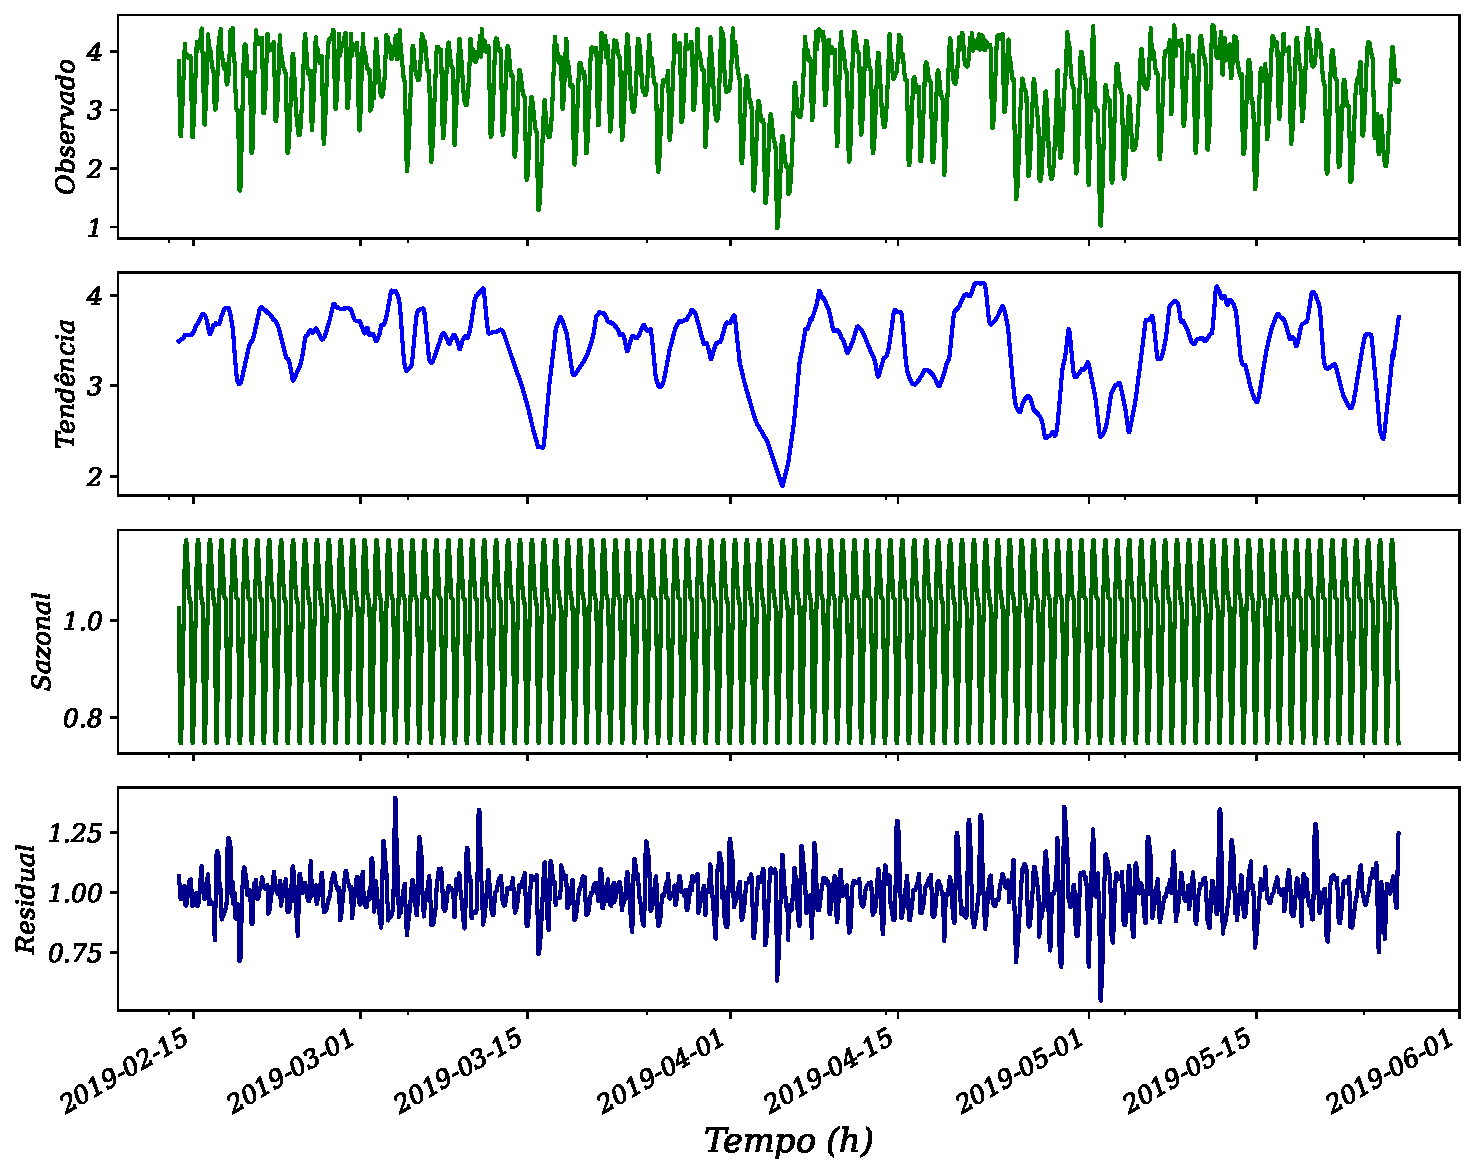
\includegraphics[width=0.8\linewidth]{Resultados/Figuras/STL}
		
	
	
\end{figure}






